\documentclass{book}
\usepackage[a4paper,top=2.5cm,bottom=2.5cm,left=2.5cm,right=2.5cm]{geometry}
\usepackage{makeidx}
\usepackage{natbib}
\usepackage{graphicx}
\usepackage{multicol}
\usepackage{float}
\usepackage{listings}
\usepackage{color}
\usepackage{ifthen}
\usepackage[table]{xcolor}
\usepackage{textcomp}
\usepackage{alltt}
\usepackage{ifpdf}
\ifpdf
\usepackage[pdftex,
            pagebackref=true,
            colorlinks=true,
            linkcolor=blue,
            unicode
           ]{hyperref}
\else
\usepackage[ps2pdf,
            pagebackref=true,
            colorlinks=true,
            linkcolor=blue,
            unicode
           ]{hyperref}
\usepackage{pspicture}
\fi
\usepackage[utf8]{inputenc}
\usepackage{mathptmx}
\usepackage[scaled=.90]{helvet}
\usepackage{courier}
\usepackage{sectsty}
\usepackage{amssymb}
\usepackage[titles]{tocloft}
\usepackage{doxygen}
\lstset{language=C++,inputencoding=utf8,basicstyle=\footnotesize,breaklines=true,breakatwhitespace=true,tabsize=4,numbers=left }
\makeindex
\setcounter{tocdepth}{3}
\renewcommand{\footrulewidth}{0.4pt}
\renewcommand{\familydefault}{\sfdefault}
\hfuzz=15pt
\setlength{\emergencystretch}{15pt}
\hbadness=750
\tolerance=750
\begin{document}
\hypersetup{pageanchor=false,citecolor=blue}
\begin{titlepage}
\vspace*{7cm}
\begin{center}
{\Large Un\-Banco \\[1ex]\large 1.\-0 }\\
\vspace*{1cm}
{\large Generated by Doxygen 1.8.3.1}\\
\vspace*{0.5cm}
{\small Fri May 17 2013 01:15:32}\\
\end{center}
\end{titlepage}
\clearemptydoublepage
\pagenumbering{roman}
\tableofcontents
\clearemptydoublepage
\pagenumbering{arabic}
\hypersetup{pageanchor=true,citecolor=blue}
\chapter{Hierarchical Index}
\section{Class Hierarchy}
This inheritance list is sorted roughly, but not completely, alphabetically\-:\begin{DoxyCompactList}
\item \contentsline{section}{Account}{\pageref{d7/d10/classAccount}}{}
\item \contentsline{section}{Main\-Interface}{\pageref{d2/da2/classMainInterface}}{}
\begin{DoxyCompactList}
\item \contentsline{section}{Main\-Adm\-Menu}{\pageref{d9/d86/classMainAdmMenu}}{}
\item \contentsline{section}{Main\-Cus\-Menu}{\pageref{dc/d35/classMainCusMenu}}{}
\item \contentsline{section}{Main\-Login}{\pageref{db/df3/classMainLogin}}{}
\item \contentsline{section}{Main\-Man\-Menu}{\pageref{d0/d1d/classMainManMenu}}{}
\end{DoxyCompactList}
\item \contentsline{section}{Payment}{\pageref{d5/d5e/classPayment}}{}
\item \contentsline{section}{Pers\-Error}{\pageref{da/dcf/classPersError}}{}
\item \contentsline{section}{Test$<$ info\-Type, class\-Type $>$}{\pageref{df/da6/classTest}}{}
\item \contentsline{section}{Transac\-Adm}{\pageref{da/deb/classTransacAdm}}{}
\item \contentsline{section}{Unit\-Base$<$ base\-Type $>$}{\pageref{d5/db5/classUnitBase}}{}
\item \contentsline{section}{Unit\-Base$<$ bool $>$}{\pageref{d5/db5/classUnitBase}}{}
\begin{DoxyCompactList}
\item \contentsline{section}{Usr\-Type}{\pageref{d1/dd4/classUsrType}}{}
\end{DoxyCompactList}
\item \contentsline{section}{Unit\-Base$<$ float $>$}{\pageref{d5/db5/classUnitBase}}{}
\begin{DoxyCompactList}
\item \contentsline{section}{Money}{\pageref{d7/d9a/classMoney}}{}
\end{DoxyCompactList}
\item \contentsline{section}{Unit\-Base$<$ int $>$}{\pageref{d5/db5/classUnitBase}}{}
\begin{DoxyCompactList}
\item \contentsline{section}{Acc\-Number}{\pageref{df/d00/classAccNumber}}{}
\item \contentsline{section}{Pay\-Code}{\pageref{d0/d34/classPayCode}}{}
\item \contentsline{section}{Pay\-Day}{\pageref{dc/d17/classPayDay}}{}
\item \contentsline{section}{Usr\-Id}{\pageref{d8/dc7/classUsrId}}{}
\item \contentsline{section}{Usr\-Matric}{\pageref{d4/d69/classUsrMatric}}{}
\end{DoxyCompactList}
\item \contentsline{section}{Unit\-Base$<$ string $>$}{\pageref{d5/db5/classUnitBase}}{}
\begin{DoxyCompactList}
\item \contentsline{section}{Usr\-Name}{\pageref{da/df7/classUsrName}}{}
\item \contentsline{section}{Usr\-Password}{\pageref{d9/d39/classUsrPassword}}{}
\end{DoxyCompactList}
\item \contentsline{section}{User}{\pageref{d9/dc0/classUser}}{}
\begin{DoxyCompactList}
\item \contentsline{section}{Customer}{\pageref{d9/d12/classCustomer}}{}
\item \contentsline{section}{Manager}{\pageref{dd/dcd/classManager}}{}
\end{DoxyCompactList}
\item \contentsline{section}{User\-Adm}{\pageref{de/dac/classUserAdm}}{}
\item \contentsline{section}{User\-Login}{\pageref{d4/de1/classUserLogin}}{}
\begin{DoxyCompactList}
\item \contentsline{section}{Stub}{\pageref{df/d32/classStub}}{}
\end{DoxyCompactList}
\item \contentsline{section}{Window}{\pageref{dc/dc4/classWindow}}{}
\begin{DoxyCompactList}
\item \contentsline{section}{Textual}{\pageref{de/da3/classTextual}}{}
\end{DoxyCompactList}
\end{DoxyCompactList}

\chapter{Class Index}
\section{Class List}
Here are the classes, structs, unions and interfaces with brief descriptions\-:\begin{DoxyCompactList}
\item\contentsline{section}{\hyperlink{classAccNumber}{Acc\-Number} \\*Define o número da conta de um \hyperlink{classCustomer}{Customer} (Cliente) }{\pageref{classAccNumber}}{}
\item\contentsline{section}{\hyperlink{classAccount}{Account} \\*Conta; Onde ficarão armazenados os dados de conta de um cliente }{\pageref{classAccount}}{}
\item\contentsline{section}{\hyperlink{classCustomer}{Customer} \\*Cliente; Onde ficarão armazenados os dados do usuário padrão do sistema }{\pageref{classCustomer}}{}
\item\contentsline{section}{\hyperlink{classManager}{Manager} \\*Gerente; Onde ficarão armazenados os dados de usuários com privilégios administrativos sobre o sistema }{\pageref{classManager}}{}
\item\contentsline{section}{\hyperlink{classMoney}{Money} \\*Define o limite da conta de um \hyperlink{classCustomer}{Customer} (Cliente) }{\pageref{classMoney}}{}
\item\contentsline{section}{\hyperlink{classPayCode}{Pay\-Code} \\*Define um número de identificação para cada pagamento }{\pageref{classPayCode}}{}
\item\contentsline{section}{\hyperlink{classPayDay}{Pay\-Day} \\*Define a data do pagamento }{\pageref{classPayDay}}{}
\item\contentsline{section}{\hyperlink{classPayment}{Payment} \\*Pagamento; Onde ficarão armazenados dados sobre pagamentos a serem realizados }{\pageref{classPayment}}{}
\item\contentsline{section}{\hyperlink{classTest}{Test$<$ info\-Type, class\-Type $>$} }{\pageref{classTest}}{}
\item\contentsline{section}{\hyperlink{classUnitBase}{Unit\-Base$<$ base\-Type $>$} \\*A base de derivação de todas as classes de tipos básicos }{\pageref{classUnitBase}}{}
\item\contentsline{section}{\hyperlink{classUser}{User} \\*Usuário; Base de derivação das classes \hyperlink{classCustomer}{Customer} e \hyperlink{classManager}{Manager} }{\pageref{classUser}}{}
\item\contentsline{section}{\hyperlink{classUsrId}{Usr\-Id} \\*Define o I\-D de um \hyperlink{classCustomer}{Customer} }{\pageref{classUsrId}}{}
\item\contentsline{section}{\hyperlink{classUsrMatric}{Usr\-Matric} \\*Define a matrícula de um \hyperlink{classManager}{Manager} }{\pageref{classUsrMatric}}{}
\item\contentsline{section}{\hyperlink{classUsrName}{Usr\-Name} \\*Define o nome de um \hyperlink{classUser}{User} (\hyperlink{classCustomer}{Customer} ou \hyperlink{classManager}{Manager}) }{\pageref{classUsrName}}{}
\item\contentsline{section}{\hyperlink{classUsrPassword}{Usr\-Password} \\*Define a senha de um \hyperlink{classUser}{User} (\hyperlink{classCustomer}{Customer} ou \hyperlink{classManager}{Manager}) }{\pageref{classUsrPassword}}{}
\item\contentsline{section}{\hyperlink{classUsrType}{Usr\-Type} \\*Codifica tipos de conta }{\pageref{classUsrType}}{}
\end{DoxyCompactList}

\chapter{Class Documentation}
\hypertarget{classAccNumber}{\section{Acc\-Number Class Reference}
\label{classAccNumber}\index{Acc\-Number@{Acc\-Number}}
}


Define o número da conta de um Customer (Cliente).  




{\ttfamily \#include $<$Base\-Unit.\-h$>$}

Inheritance diagram for Acc\-Number\-:\begin{figure}[H]
\begin{center}
\leavevmode
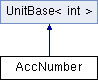
\includegraphics[height=2.000000cm]{classAccNumber}
\end{center}
\end{figure}
\subsection*{Public Member Functions}
\begin{DoxyCompactItemize}
\item 
\hypertarget{classAccNumber_a11a8a2ea0849a83365960758a5ff3362}{{\bfseries Acc\-Number} (int)  throw (invalid\-\_\-argument)}\label{classAccNumber_a11a8a2ea0849a83365960758a5ff3362}

\end{DoxyCompactItemize}
\subsection*{Additional Inherited Members}


\subsection{Detailed Description}
Define o número da conta de um Customer (Cliente). 

Este tipo básico tem a função de atribuir a cada conta um numero unico, identificando-\/a. 

The documentation for this class was generated from the following files\-:\begin{DoxyCompactItemize}
\item 
Base\-Unit.\-h\item 
Base\-Unit.\-cpp\end{DoxyCompactItemize}

\hypertarget{classAccount}{\section{Account Class Reference}
\label{d7/d10/classAccount}\index{Account@{Account}}
}


Conta; Onde ficarão armazenados os dados de conta de um cliente.  




{\ttfamily \#include $<$Entity\-Unit.\-h$>$}

\subsection*{Public Member Functions}
\begin{DoxyCompactItemize}
\item 
\hyperlink{classAccount_a94113be123fc89c3de8461cbb8251c83}{Account} (const \hyperlink{classAccNumber}{Acc\-Number} \&, const \hyperlink{classUsrType}{Acc\-Type} \&, const \hyperlink{classMoney}{Money} \&, const \hyperlink{classMoney}{Money} \&, const \hyperlink{classUsrId}{Usr\-Id} \&)
\begin{DoxyCompactList}\small\item\em Construtor base de \hyperlink{classAccount}{Account}. \end{DoxyCompactList}\item 
\hyperlink{classAccNumber}{Acc\-Number} \hyperlink{classAccount_a74f26f24e13e66a055bb8441dfb3d881}{get\-Acc\-Number} () const 
\begin{DoxyCompactList}\small\item\em Método que retorna o valor contido no atributo acc\-Number. \end{DoxyCompactList}\item 
void \hyperlink{classAccount_a3e669090168f13d2a8269af456546a1e}{set\-Acc\-Number} (const \hyperlink{classAccNumber}{Acc\-Number} \&)
\begin{DoxyCompactList}\small\item\em Método que define o valor do atributo acc\-Number. \end{DoxyCompactList}\item 
\hyperlink{classUsrType}{Acc\-Type} \hyperlink{classAccount_a34e1f7e507d7abdf575e4833d6f8d36b}{get\-Acc\-Type} () const 
\begin{DoxyCompactList}\small\item\em Método que retorna o valor contido no atributo acc\-Type. \end{DoxyCompactList}\item 
void \hyperlink{classAccount_a3a8e8aa0094b2af0496d45714f694256}{set\-Acc\-Type} (const \hyperlink{classUsrType}{Acc\-Type} \&)
\begin{DoxyCompactList}\small\item\em Método que define o valor do atributo acc\-Type. \end{DoxyCompactList}\item 
\hyperlink{classMoney}{Money} \hyperlink{classAccount_ac67a380f5f320a44f9bb464f6efd59f7}{get\-Limit} () const 
\begin{DoxyCompactList}\small\item\em Método que retorna o valor contido no atributo limit. \end{DoxyCompactList}\item 
void \hyperlink{classAccount_ada9bd7d0aee82d5b6c8f9831eb6fd8d5}{set\-Limit} (const \hyperlink{classMoney}{Money} \&)
\begin{DoxyCompactList}\small\item\em Método que define o valor do atributo limit. \end{DoxyCompactList}\item 
\hyperlink{classMoney}{Money} \hyperlink{classAccount_af9414bc748bf1923b2308544bbfd8b82}{get\-Balance} () const 
\begin{DoxyCompactList}\small\item\em Método que retorna o valor contido no atributo balance. \end{DoxyCompactList}\item 
void \hyperlink{classAccount_a0c54b27c54fd64b93d31aecdf7f3f302}{set\-Balance} (const \hyperlink{classMoney}{Money} \&)
\begin{DoxyCompactList}\small\item\em Método que define o valor do atributo balance. \end{DoxyCompactList}\item 
\hyperlink{classUsrId}{Usr\-Id} \hyperlink{classAccount_a59a83e5c5142f79402e79a8d42b36aed}{get\-Usr\-Id} () const 
\begin{DoxyCompactList}\small\item\em Método que retorna o valor contido no atributo usr\-Id. \end{DoxyCompactList}\item 
void \hyperlink{classAccount_a97146ede9747001294bcd41c74abd67a}{set\-Usr\-Id} (const \hyperlink{classUsrId}{Usr\-Id} \&)
\begin{DoxyCompactList}\small\item\em Método que define o valor do atributo usr\-Id. \end{DoxyCompactList}\end{DoxyCompactItemize}


\subsection{Detailed Description}
Conta; Onde ficarão armazenados os dados de conta de um cliente. 

Através de uma conta é possível acessar o módulo de Transações. 

\subsection{Constructor \& Destructor Documentation}
\hypertarget{classAccount_a94113be123fc89c3de8461cbb8251c83}{\index{Account@{Account}!Account@{Account}}
\index{Account@{Account}!Account@{Account}}
\subsubsection[{Account}]{\setlength{\rightskip}{0pt plus 5cm}Account\-::\-Account (
\begin{DoxyParamCaption}
\item[{const {\bf Acc\-Number} \&}]{acc\-Number, }
\item[{const {\bf Acc\-Type} \&}]{acc\-Type, }
\item[{const {\bf Money} \&}]{limit, }
\item[{const {\bf Money} \&}]{balance, }
\item[{const {\bf Usr\-Id} \&}]{usr\-Id}
\end{DoxyParamCaption}
)}}\label{d7/d10/classAccount_a94113be123fc89c3de8461cbb8251c83}


Construtor base de \hyperlink{classAccount}{Account}. 

Define os valores internos da classe automaticamente. 

\subsection{Member Function Documentation}
\hypertarget{classAccount_a74f26f24e13e66a055bb8441dfb3d881}{\index{Account@{Account}!get\-Acc\-Number@{get\-Acc\-Number}}
\index{get\-Acc\-Number@{get\-Acc\-Number}!Account@{Account}}
\subsubsection[{get\-Acc\-Number}]{\setlength{\rightskip}{0pt plus 5cm}{\bf Acc\-Number} Account\-::get\-Acc\-Number (
\begin{DoxyParamCaption}
{}
\end{DoxyParamCaption}
) const\hspace{0.3cm}{\ttfamily [inline]}}}\label{d7/d10/classAccount_a74f26f24e13e66a055bb8441dfb3d881}


Método que retorna o valor contido no atributo acc\-Number. 

O valor será retornado e o atributo não será modificado. \hypertarget{classAccount_a34e1f7e507d7abdf575e4833d6f8d36b}{\index{Account@{Account}!get\-Acc\-Type@{get\-Acc\-Type}}
\index{get\-Acc\-Type@{get\-Acc\-Type}!Account@{Account}}
\subsubsection[{get\-Acc\-Type}]{\setlength{\rightskip}{0pt plus 5cm}{\bf Acc\-Type} Account\-::get\-Acc\-Type (
\begin{DoxyParamCaption}
{}
\end{DoxyParamCaption}
) const\hspace{0.3cm}{\ttfamily [inline]}}}\label{d7/d10/classAccount_a34e1f7e507d7abdf575e4833d6f8d36b}


Método que retorna o valor contido no atributo acc\-Type. 

O valor será retornado e o atributo não será modificado. \hypertarget{classAccount_af9414bc748bf1923b2308544bbfd8b82}{\index{Account@{Account}!get\-Balance@{get\-Balance}}
\index{get\-Balance@{get\-Balance}!Account@{Account}}
\subsubsection[{get\-Balance}]{\setlength{\rightskip}{0pt plus 5cm}{\bf Money} Account\-::get\-Balance (
\begin{DoxyParamCaption}
{}
\end{DoxyParamCaption}
) const\hspace{0.3cm}{\ttfamily [inline]}}}\label{d7/d10/classAccount_af9414bc748bf1923b2308544bbfd8b82}


Método que retorna o valor contido no atributo balance. 

O valor será retornado e o atributo não será modificado. \hypertarget{classAccount_ac67a380f5f320a44f9bb464f6efd59f7}{\index{Account@{Account}!get\-Limit@{get\-Limit}}
\index{get\-Limit@{get\-Limit}!Account@{Account}}
\subsubsection[{get\-Limit}]{\setlength{\rightskip}{0pt plus 5cm}{\bf Money} Account\-::get\-Limit (
\begin{DoxyParamCaption}
{}
\end{DoxyParamCaption}
) const\hspace{0.3cm}{\ttfamily [inline]}}}\label{d7/d10/classAccount_ac67a380f5f320a44f9bb464f6efd59f7}


Método que retorna o valor contido no atributo limit. 

O valor será retornado e o atributo não será modificado. \hypertarget{classAccount_a59a83e5c5142f79402e79a8d42b36aed}{\index{Account@{Account}!get\-Usr\-Id@{get\-Usr\-Id}}
\index{get\-Usr\-Id@{get\-Usr\-Id}!Account@{Account}}
\subsubsection[{get\-Usr\-Id}]{\setlength{\rightskip}{0pt plus 5cm}{\bf Usr\-Id} Account\-::get\-Usr\-Id (
\begin{DoxyParamCaption}
{}
\end{DoxyParamCaption}
) const\hspace{0.3cm}{\ttfamily [inline]}}}\label{d7/d10/classAccount_a59a83e5c5142f79402e79a8d42b36aed}


Método que retorna o valor contido no atributo usr\-Id. 

O valor será retornado e o atributo não será modificado. \hypertarget{classAccount_a3e669090168f13d2a8269af456546a1e}{\index{Account@{Account}!set\-Acc\-Number@{set\-Acc\-Number}}
\index{set\-Acc\-Number@{set\-Acc\-Number}!Account@{Account}}
\subsubsection[{set\-Acc\-Number}]{\setlength{\rightskip}{0pt plus 5cm}void Account\-::set\-Acc\-Number (
\begin{DoxyParamCaption}
\item[{const {\bf Acc\-Number} \&}]{acc\-Number}
\end{DoxyParamCaption}
)}}\label{d7/d10/classAccount_a3e669090168f13d2a8269af456546a1e}


Método que define o valor do atributo acc\-Number. 

\hypertarget{classAccount_a3a8e8aa0094b2af0496d45714f694256}{\index{Account@{Account}!set\-Acc\-Type@{set\-Acc\-Type}}
\index{set\-Acc\-Type@{set\-Acc\-Type}!Account@{Account}}
\subsubsection[{set\-Acc\-Type}]{\setlength{\rightskip}{0pt plus 5cm}void Account\-::set\-Acc\-Type (
\begin{DoxyParamCaption}
\item[{const {\bf Acc\-Type} \&}]{acc\-Type}
\end{DoxyParamCaption}
)}}\label{d7/d10/classAccount_a3a8e8aa0094b2af0496d45714f694256}


Método que define o valor do atributo acc\-Type. 

\hypertarget{classAccount_a0c54b27c54fd64b93d31aecdf7f3f302}{\index{Account@{Account}!set\-Balance@{set\-Balance}}
\index{set\-Balance@{set\-Balance}!Account@{Account}}
\subsubsection[{set\-Balance}]{\setlength{\rightskip}{0pt plus 5cm}void Account\-::set\-Balance (
\begin{DoxyParamCaption}
\item[{const {\bf Money} \&}]{balance}
\end{DoxyParamCaption}
)}}\label{d7/d10/classAccount_a0c54b27c54fd64b93d31aecdf7f3f302}


Método que define o valor do atributo balance. 

\hypertarget{classAccount_ada9bd7d0aee82d5b6c8f9831eb6fd8d5}{\index{Account@{Account}!set\-Limit@{set\-Limit}}
\index{set\-Limit@{set\-Limit}!Account@{Account}}
\subsubsection[{set\-Limit}]{\setlength{\rightskip}{0pt plus 5cm}void Account\-::set\-Limit (
\begin{DoxyParamCaption}
\item[{const {\bf Money} \&}]{limit}
\end{DoxyParamCaption}
)}}\label{d7/d10/classAccount_ada9bd7d0aee82d5b6c8f9831eb6fd8d5}


Método que define o valor do atributo limit. 

\hypertarget{classAccount_a97146ede9747001294bcd41c74abd67a}{\index{Account@{Account}!set\-Usr\-Id@{set\-Usr\-Id}}
\index{set\-Usr\-Id@{set\-Usr\-Id}!Account@{Account}}
\subsubsection[{set\-Usr\-Id}]{\setlength{\rightskip}{0pt plus 5cm}void Account\-::set\-Usr\-Id (
\begin{DoxyParamCaption}
\item[{const {\bf Usr\-Id} \&}]{usr\-Id}
\end{DoxyParamCaption}
)}}\label{d7/d10/classAccount_a97146ede9747001294bcd41c74abd67a}


Método que define o valor do atributo usr\-Id. 



The documentation for this class was generated from the following files\-:\begin{DoxyCompactItemize}
\item 
Entity\-Unit.\-h\item 
Entity\-Unit.\-cpp\end{DoxyCompactItemize}

\hypertarget{classCustomer}{\subsection{Customer Class Reference}
\label{d9/d12/classCustomer}\index{Customer@{Customer}}
}


Cliente; Onde ficarão armazenados os dados do usuário padrão do sistema.  




{\ttfamily \#include $<$Entity\-Unit.\-h$>$}

Inheritance diagram for Customer\-:\begin{figure}[H]
\begin{center}
\leavevmode
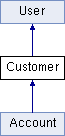
\includegraphics[height=2.000000cm]{d9/d12/classCustomer}
\end{center}
\end{figure}
\subsubsection*{Public Member Functions}
\begin{DoxyCompactItemize}
\item 
\hyperlink{classCustomer_a3f3be282d21b234e1e72f645d8fdc362}{Customer} (const \hyperlink{classUsrName}{Usr\-Name} \&, const \hyperlink{classUsrPassword}{Usr\-Password} \&, const \hyperlink{classUsrId}{Usr\-Id} \&)
\begin{DoxyCompactList}\small\item\em Construtor base de \hyperlink{classCustomer}{Customer}. \end{DoxyCompactList}\item 
\hyperlink{classUsrId}{Usr\-Id} \hyperlink{classCustomer_a76d325591ef27599cb1d7f3e4b77b8d4}{get\-Usr\-Id} () const 
\begin{DoxyCompactList}\small\item\em Método que recupera o valor contido no campo usr\-Id. \end{DoxyCompactList}\item 
void \hyperlink{classCustomer_a89b74269a4750193d61b305b13df82fa}{set\-Usr\-Id} (const \hyperlink{classUsrId}{Usr\-Id} \&)
\begin{DoxyCompactList}\small\item\em Método que define o valor do atributo usr\-Id. \end{DoxyCompactList}\end{DoxyCompactItemize}
\subsubsection*{Additional Inherited Members}


\subsubsection{Detailed Description}
Cliente; Onde ficarão armazenados os dados do usuário padrão do sistema. 

O \hyperlink{classCustomer}{Customer} (Cliente) terá acesso a uma ou mais contas através de um \hyperlink{classUsrId}{Usr\-Id} único. Através dessa(s) conta(s), é capaz de realizar transações. 

Definition at line 40 of file Entity\-Unit.\-h.



\subsubsection{Constructor \& Destructor Documentation}
\hypertarget{classCustomer_a3f3be282d21b234e1e72f645d8fdc362}{\index{Customer@{Customer}!Customer@{Customer}}
\index{Customer@{Customer}!Customer@{Customer}}
\paragraph[{Customer}]{\setlength{\rightskip}{0pt plus 5cm}Customer\-::\-Customer (
\begin{DoxyParamCaption}
\item[{const {\bf Usr\-Name} \&}]{name, }
\item[{const {\bf Usr\-Password} \&}]{password, }
\item[{const {\bf Usr\-Id} \&}]{usr\-Id}
\end{DoxyParamCaption}
)}}\label{d9/d12/classCustomer_a3f3be282d21b234e1e72f645d8fdc362}


Construtor base de \hyperlink{classCustomer}{Customer}. 

Define os valores internos da classe automaticamente. 

Definition at line 17 of file Entity\-Unit.\-cpp.



\subsubsection{Member Function Documentation}
\hypertarget{classCustomer_a76d325591ef27599cb1d7f3e4b77b8d4}{\index{Customer@{Customer}!get\-Usr\-Id@{get\-Usr\-Id}}
\index{get\-Usr\-Id@{get\-Usr\-Id}!Customer@{Customer}}
\paragraph[{get\-Usr\-Id}]{\setlength{\rightskip}{0pt plus 5cm}{\bf Usr\-Id} Customer\-::get\-Usr\-Id (
\begin{DoxyParamCaption}
{}
\end{DoxyParamCaption}
) const\hspace{0.3cm}{\ttfamily [inline]}}}\label{d9/d12/classCustomer_a76d325591ef27599cb1d7f3e4b77b8d4}


Método que recupera o valor contido no campo usr\-Id. 

O valor é retornado, e o atributo não é modificado no processo. 

Definition at line 59 of file Entity\-Unit.\-h.

\hypertarget{classCustomer_a89b74269a4750193d61b305b13df82fa}{\index{Customer@{Customer}!set\-Usr\-Id@{set\-Usr\-Id}}
\index{set\-Usr\-Id@{set\-Usr\-Id}!Customer@{Customer}}
\paragraph[{set\-Usr\-Id}]{\setlength{\rightskip}{0pt plus 5cm}void Customer\-::set\-Usr\-Id (
\begin{DoxyParamCaption}
\item[{const {\bf Usr\-Id} \&}]{usr\-Id}
\end{DoxyParamCaption}
)}}\label{d9/d12/classCustomer_a89b74269a4750193d61b305b13df82fa}


Método que define o valor do atributo usr\-Id. 



Definition at line 24 of file Entity\-Unit.\-cpp.



The documentation for this class was generated from the following files\-:\begin{DoxyCompactItemize}
\item 
Entity\-Unit.\-h\item 
Entity\-Unit.\-cpp\end{DoxyCompactItemize}

\hypertarget{classManager}{\section{Manager Class Reference}
\label{classManager}\index{Manager@{Manager}}
}


Gerente; Onde ficarão armazenados os dados de usuários com privilégios administrativos sobre o sistema.  




{\ttfamily \#include $<$Entity\-Unit.\-h$>$}

Inheritance diagram for Manager\-:\begin{figure}[H]
\begin{center}
\leavevmode
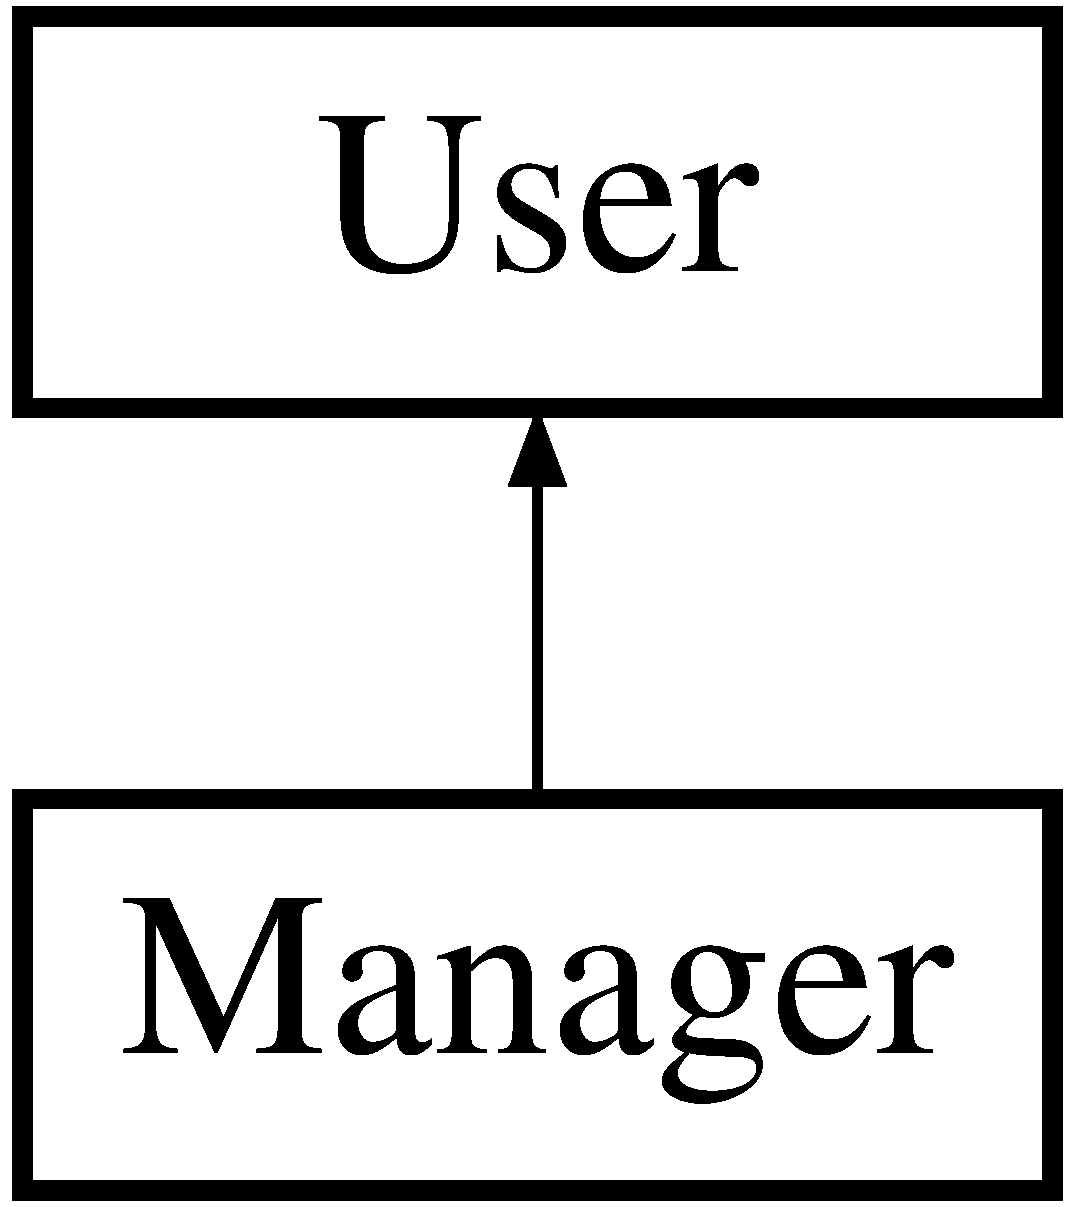
\includegraphics[height=2.000000cm]{classManager}
\end{center}
\end{figure}
\subsection*{Public Member Functions}
\begin{DoxyCompactItemize}
\item 
\hypertarget{classManager_ad2ee8089f5e80bc03fabcf9a493d045b}{{\bfseries Manager} (const \hyperlink{classUsrName}{Usr\-Name} \&, const \hyperlink{classUsrPassword}{Usr\-Password} \&, const \hyperlink{classUsrType}{Man\-Type} \&, const \hyperlink{classUsrMatric}{Usr\-Matric} \&)  throw (invalid\-\_\-argument)}\label{classManager_ad2ee8089f5e80bc03fabcf9a493d045b}

\item 
\hypertarget{classManager_a255ac6a7e2112631001296fa8db3811b}{\hyperlink{classUsrType}{Man\-Type} {\bfseries get\-Man\-Type} () const }\label{classManager_a255ac6a7e2112631001296fa8db3811b}

\item 
\hypertarget{classManager_a3d4e9cb6cc0e8d9be47fcc086b4e584e}{void {\bfseries set\-Man\-Type} (const \hyperlink{classUsrType}{Man\-Type} \&)}\label{classManager_a3d4e9cb6cc0e8d9be47fcc086b4e584e}

\item 
\hypertarget{classManager_a462f3704b016b57e087db417df73f07a}{\hyperlink{classUsrMatric}{Usr\-Matric} {\bfseries get\-Usr\-Matric} () const }\label{classManager_a462f3704b016b57e087db417df73f07a}

\item 
\hypertarget{classManager_a93309a0dde84dd0b5fe90d9e1da49822}{void {\bfseries set\-Usr\-Matric} (const \hyperlink{classUsrMatric}{Usr\-Matric} \&)}\label{classManager_a93309a0dde84dd0b5fe90d9e1da49822}

\end{DoxyCompactItemize}
\subsection*{Additional Inherited Members}


\subsection{Detailed Description}
Gerente; Onde ficarão armazenados os dados de usuários com privilégios administrativos sobre o sistema. 

Através desta classe é possível acessar o módulo de Usr\-Manage e modificar dados de outros usuários. 

The documentation for this class was generated from the following files\-:\begin{DoxyCompactItemize}
\item 
Entity\-Unit.\-h\item 
Entity\-Unit.\-cpp\end{DoxyCompactItemize}

\hypertarget{classMoney}{\section{Money Class Reference}
\label{classMoney}\index{Money@{Money}}
}


Define o limite da conta de um \hyperlink{classCustomer}{Customer} (Cliente).  




{\ttfamily \#include $<$Base\-Unit.\-h$>$}

Inheritance diagram for Money\-:\begin{figure}[H]
\begin{center}
\leavevmode
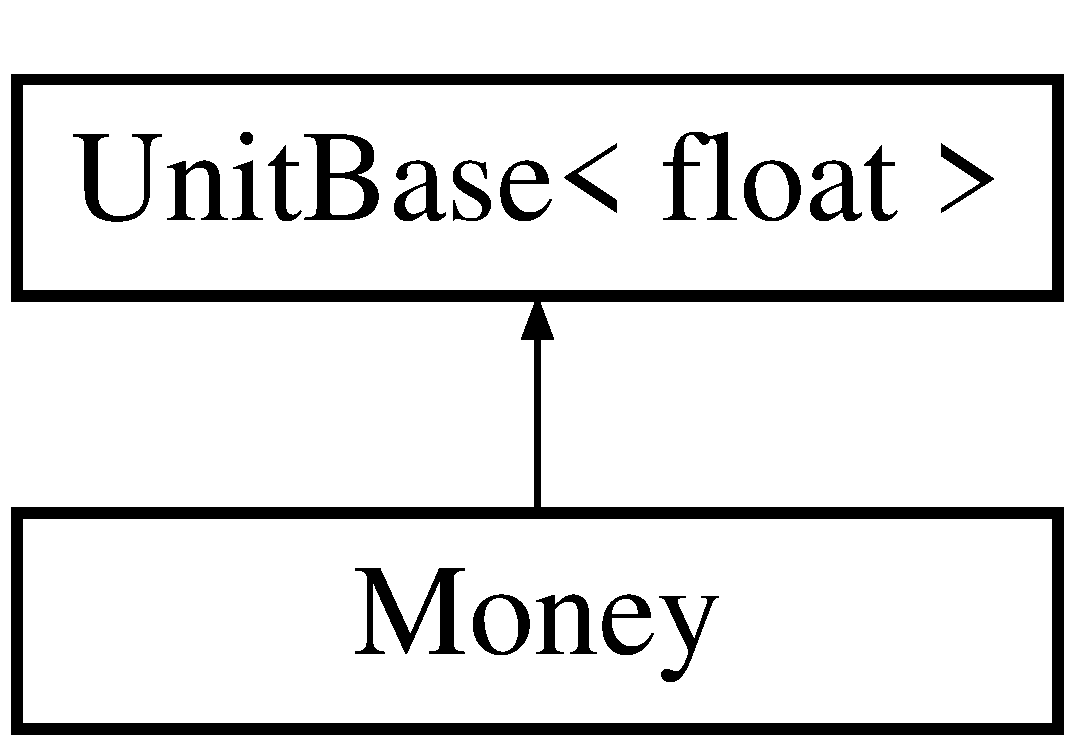
\includegraphics[height=2.000000cm]{classMoney}
\end{center}
\end{figure}
\subsection*{Public Member Functions}
\begin{DoxyCompactItemize}
\item 
\hypertarget{classMoney_a33986736e7432883ebd61584815b6681}{{\bfseries Money} (const float \&)  throw (invalid\-\_\-argument)}\label{classMoney_a33986736e7432883ebd61584815b6681}

\end{DoxyCompactItemize}
\subsection*{Additional Inherited Members}


\subsection{Detailed Description}
Define o limite da conta de um \hyperlink{classCustomer}{Customer} (Cliente). 

Atribui a cada conta um limite, limitando a utilização do crédito junto ao banco. 

The documentation for this class was generated from the following files\-:\begin{DoxyCompactItemize}
\item 
Base\-Unit.\-h\item 
Base\-Unit.\-cpp\end{DoxyCompactItemize}

\hypertarget{classPayCode}{\section{Pay\-Code Class Reference}
\label{classPayCode}\index{Pay\-Code@{Pay\-Code}}
}


Define um número de identificação para cada pagamento.  




{\ttfamily \#include $<$Base\-Unit.\-h$>$}

Inheritance diagram for Pay\-Code\-:\begin{figure}[H]
\begin{center}
\leavevmode
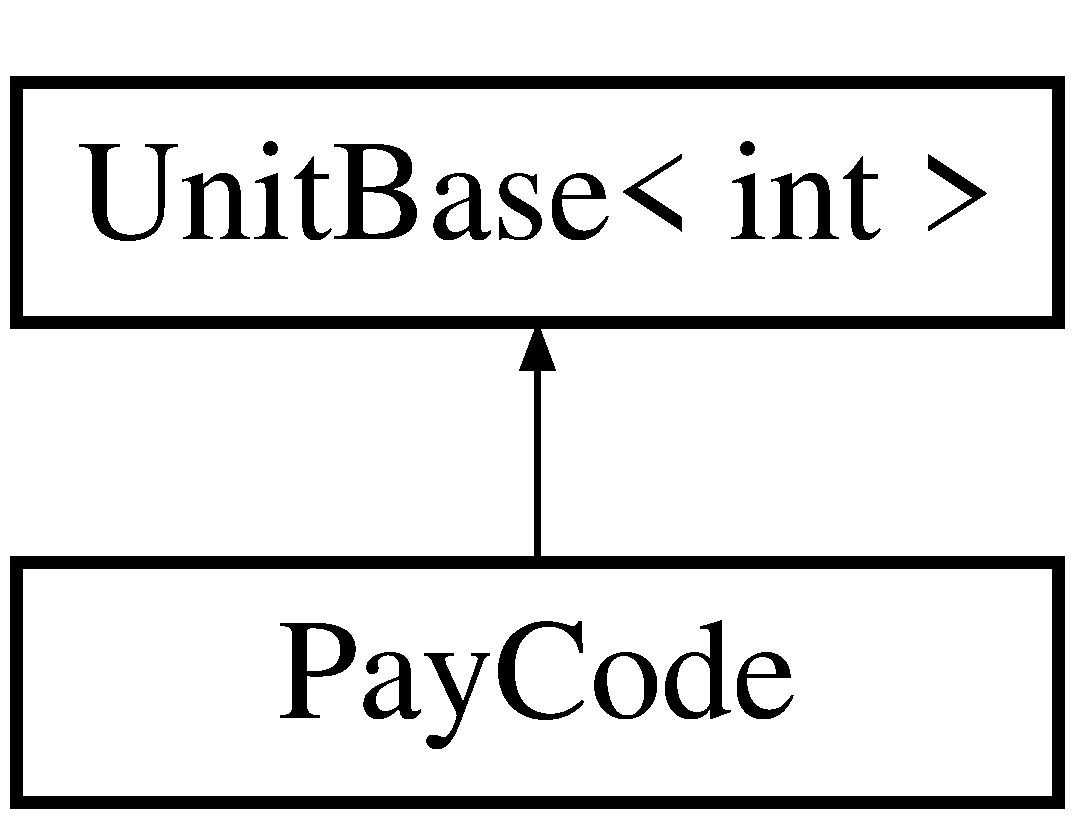
\includegraphics[height=2.000000cm]{classPayCode}
\end{center}
\end{figure}
\subsection*{Public Member Functions}
\begin{DoxyCompactItemize}
\item 
\hypertarget{classPayCode_a919ab6e420b9bd55e8c470ea411aa97e}{{\bfseries Pay\-Code} (const int \&)  throw (invalid\-\_\-argument)}\label{classPayCode_a919ab6e420b9bd55e8c470ea411aa97e}

\end{DoxyCompactItemize}
\subsection*{Additional Inherited Members}


\subsection{Detailed Description}
Define um número de identificação para cada pagamento. 

Atribui a cada pagamento um código, de forma a identificá-\/lo. 

The documentation for this class was generated from the following files\-:\begin{DoxyCompactItemize}
\item 
Base\-Unit.\-h\item 
Base\-Unit.\-cpp\end{DoxyCompactItemize}

\hypertarget{classPayDay}{\subsection{Pay\-Day Class Reference}
\label{dc/d17/classPayDay}\index{Pay\-Day@{Pay\-Day}}
}


Define a data do pagamento.  




{\ttfamily \#include $<$Base\-Unit.\-h$>$}

Inheritance diagram for Pay\-Day\-:\begin{figure}[H]
\begin{center}
\leavevmode
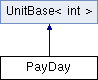
\includegraphics[height=2.000000cm]{dc/d17/classPayDay}
\end{center}
\end{figure}
\subsubsection*{Public Member Functions}
\begin{DoxyCompactItemize}
\item 
\hyperlink{classPayDay_a6da36cea0b2ac9a53106552aad00996a}{Pay\-Day} ()
\begin{DoxyCompactList}\small\item\em Construtor padrão de \hyperlink{classPayDay}{Pay\-Day}. \end{DoxyCompactList}\item 
\hyperlink{classPayDay_aa11abdfdb58bbd93f68bc02a7496e1c4}{Pay\-Day} (const int \&)  throw (invalid\-\_\-argument)
\begin{DoxyCompactList}\small\item\em Construtor base de \hyperlink{classPayDay}{Pay\-Day}. \end{DoxyCompactList}\item 
int \hyperlink{classPayDay_a297ce892f49aa9f3a504d514f171ed1d}{day} ()
\begin{DoxyCompactList}\small\item\em Método que retorna o dia contido na data. \end{DoxyCompactList}\item 
int \hyperlink{classPayDay_ada65e8834c142a95cd35ca2b399fbcde}{month} ()
\begin{DoxyCompactList}\small\item\em Método que retorna o mês contido na data. \end{DoxyCompactList}\item 
int \hyperlink{classPayDay_a962960925f9e6eaaac0fef5eb96849ec}{year} ()
\begin{DoxyCompactList}\small\item\em Método que retorna o ano contido na data. \end{DoxyCompactList}\end{DoxyCompactItemize}
\subsubsection*{Additional Inherited Members}


\subsubsection{Detailed Description}
Define a data do pagamento. 

Guarda a data de um pagamento num inteiro de formato D\-D\-M\-M\-A\-A\-A\-A. Dia, mês e ano devem ser acessados através dos atributos day, month, year. 

Definition at line 196 of file Base\-Unit.\-h.



\subsubsection{Constructor \& Destructor Documentation}
\hypertarget{classPayDay_a6da36cea0b2ac9a53106552aad00996a}{\index{Pay\-Day@{Pay\-Day}!Pay\-Day@{Pay\-Day}}
\index{Pay\-Day@{Pay\-Day}!PayDay@{Pay\-Day}}
\paragraph[{Pay\-Day}]{\setlength{\rightskip}{0pt plus 5cm}Pay\-Day\-::\-Pay\-Day (
\begin{DoxyParamCaption}
{}
\end{DoxyParamCaption}
)}}\label{dc/d17/classPayDay_a6da36cea0b2ac9a53106552aad00996a}


Construtor padrão de \hyperlink{classPayDay}{Pay\-Day}. 

Define o valor 0 como valor de não-\/inicialização deste tipo básico. 

Definition at line 173 of file Base\-Unit.\-cpp.

\hypertarget{classPayDay_aa11abdfdb58bbd93f68bc02a7496e1c4}{\index{Pay\-Day@{Pay\-Day}!Pay\-Day@{Pay\-Day}}
\index{Pay\-Day@{Pay\-Day}!PayDay@{Pay\-Day}}
\paragraph[{Pay\-Day}]{\setlength{\rightskip}{0pt plus 5cm}Pay\-Day\-::\-Pay\-Day (
\begin{DoxyParamCaption}
\item[{const int \&}]{date}
\end{DoxyParamCaption}
)  throw (invalid\-\_\-argument)}}\label{dc/d17/classPayDay_aa11abdfdb58bbd93f68bc02a7496e1c4}


Construtor base de \hyperlink{classPayDay}{Pay\-Day}. 

É preferível que se utilize este construtor pois ele já faz a validação automática do valor a ser definido. 

Definition at line 178 of file Base\-Unit.\-cpp.



\subsubsection{Member Function Documentation}
\hypertarget{classPayDay_a297ce892f49aa9f3a504d514f171ed1d}{\index{Pay\-Day@{Pay\-Day}!day@{day}}
\index{day@{day}!PayDay@{Pay\-Day}}
\paragraph[{day}]{\setlength{\rightskip}{0pt plus 5cm}int Pay\-Day\-::day (
\begin{DoxyParamCaption}
{}
\end{DoxyParamCaption}
)\hspace{0.3cm}{\ttfamily [inline]}}}\label{dc/d17/classPayDay_a297ce892f49aa9f3a504d514f171ed1d}


Método que retorna o dia contido na data. 

Extrai do inteiro contido no objeto o dia a que ele se refere. 

Definition at line 231 of file Base\-Unit.\-h.

\hypertarget{classPayDay_ada65e8834c142a95cd35ca2b399fbcde}{\index{Pay\-Day@{Pay\-Day}!month@{month}}
\index{month@{month}!PayDay@{Pay\-Day}}
\paragraph[{month}]{\setlength{\rightskip}{0pt plus 5cm}int Pay\-Day\-::month (
\begin{DoxyParamCaption}
{}
\end{DoxyParamCaption}
)\hspace{0.3cm}{\ttfamily [inline]}}}\label{dc/d17/classPayDay_ada65e8834c142a95cd35ca2b399fbcde}


Método que retorna o mês contido na data. 

Extrai do inteiro contido no objeto o mês a que ele se refere. 

Definition at line 226 of file Base\-Unit.\-h.

\hypertarget{classPayDay_a962960925f9e6eaaac0fef5eb96849ec}{\index{Pay\-Day@{Pay\-Day}!year@{year}}
\index{year@{year}!PayDay@{Pay\-Day}}
\paragraph[{year}]{\setlength{\rightskip}{0pt plus 5cm}int Pay\-Day\-::year (
\begin{DoxyParamCaption}
{}
\end{DoxyParamCaption}
)\hspace{0.3cm}{\ttfamily [inline]}}}\label{dc/d17/classPayDay_a962960925f9e6eaaac0fef5eb96849ec}


Método que retorna o ano contido na data. 

Extrai do inteiro contido no objeto o ano a que ele se refere. 

Definition at line 221 of file Base\-Unit.\-h.



The documentation for this class was generated from the following files\-:\begin{DoxyCompactItemize}
\item 
Base\-Unit.\-h\item 
Base\-Unit.\-cpp\end{DoxyCompactItemize}

\hypertarget{classPayment}{\section{Payment Class Reference}
\label{d5/d5e/classPayment}\index{Payment@{Payment}}
}


Pagamento; Onde ficarão armazenados dados sobre pagamentos a serem realizados.  




{\ttfamily \#include $<$Entity\-Unit.\-h$>$}

\subsection*{Public Member Functions}
\begin{DoxyCompactItemize}
\item 
\hyperlink{classPayment_a91b7742c5f9b4617e4a3bce6507cce49}{Payment} (const \hyperlink{classAccNumber}{Acc\-Number} \&, const \hyperlink{classPayDay}{Pay\-Day} \&, const \hyperlink{classMoney}{Money} \&)  throw (invalid\-\_\-argument)
\begin{DoxyCompactList}\small\item\em Construtor base de \hyperlink{classPayment}{Payment}. \end{DoxyCompactList}\item 
\hyperlink{classPayCode}{Pay\-Code} \hyperlink{classPayment_a1d71998fa33e757bb350eb40895865ae}{get\-Pay\-Code} () const 
\begin{DoxyCompactList}\small\item\em Método que recupera o valor contido no atributo pay\-Code. \end{DoxyCompactList}\item 
const \hyperlink{classPayCode}{Pay\-Code} \hyperlink{classPayment_adf458db6331e53948a473a04a0d622a4}{set\-Pay\-Code} (const \hyperlink{classPayCode}{Pay\-Code} \&)
\begin{DoxyCompactList}\small\item\em Método que define o valor no atributo pay\-Code. \end{DoxyCompactList}\item 
\hyperlink{classAccNumber}{Acc\-Number} \hyperlink{classPayment_a66c51330aef2e045884e25618a194904}{get\-Acc\-Number} () const 
\begin{DoxyCompactList}\small\item\em Método que recupera o valor contido no atributo acc\-Number. \end{DoxyCompactList}\item 
void \hyperlink{classPayment_a5d0e83f83f090acf4b33bc81f5391ca0}{set\-Acc\-Number} (const \hyperlink{classAccNumber}{Acc\-Number} \&)
\begin{DoxyCompactList}\small\item\em Método que define o valor no atributo pay\-Code. \end{DoxyCompactList}\item 
\hyperlink{classPayDay}{Pay\-Day} \hyperlink{classPayment_a22ee22d04f3f5757f115386aa3337c51}{get\-Pay\-Day} () const 
\begin{DoxyCompactList}\small\item\em Método que recupera o valor contido no atributo pay\-Day. \end{DoxyCompactList}\item 
void \hyperlink{classPayment_aaadd94e11ab24629d536809da691efc5}{set\-Pay\-Day} (const \hyperlink{classPayDay}{Pay\-Day} \&)
\begin{DoxyCompactList}\small\item\em Método que define o valor no atributo pay\-Code. \end{DoxyCompactList}\item 
\hyperlink{classMoney}{Money} \hyperlink{classPayment_a3a2d6a8dc3f6b63e924504e1994ae556}{get\-Pay\-Value} () const 
\begin{DoxyCompactList}\small\item\em Método que recupera o valor contido no atributo pay\-Value. \end{DoxyCompactList}\item 
void \hyperlink{classPayment_ace63ad77804d5a19ace50aa1a7335050}{set\-Pay\-Value} (const \hyperlink{classMoney}{Money} \&)
\begin{DoxyCompactList}\small\item\em Método que define o valor no atributo pay\-Code. \end{DoxyCompactList}\end{DoxyCompactItemize}


\subsection{Detailed Description}
Pagamento; Onde ficarão armazenados dados sobre pagamentos a serem realizados. 

Esta classe armazenará os dados de conta bem como a data agendada de pagamentos futuros. 

\subsection{Constructor \& Destructor Documentation}
\hypertarget{classPayment_a91b7742c5f9b4617e4a3bce6507cce49}{\index{Payment@{Payment}!Payment@{Payment}}
\index{Payment@{Payment}!Payment@{Payment}}
\subsubsection[{Payment}]{\setlength{\rightskip}{0pt plus 5cm}Payment\-::\-Payment (
\begin{DoxyParamCaption}
\item[{const {\bf Acc\-Number} \&}]{acc\-Number, }
\item[{const {\bf Pay\-Day} \&}]{pay\-Day, }
\item[{const {\bf Money} \&}]{pay\-Value}
\end{DoxyParamCaption}
)  throw (invalid\-\_\-argument)}}\label{d5/d5e/classPayment_a91b7742c5f9b4617e4a3bce6507cce49}


Construtor base de \hyperlink{classPayment}{Payment}. 

Define todos os atributos internos à classe automaticamente. 

\subsection{Member Function Documentation}
\hypertarget{classPayment_a66c51330aef2e045884e25618a194904}{\index{Payment@{Payment}!get\-Acc\-Number@{get\-Acc\-Number}}
\index{get\-Acc\-Number@{get\-Acc\-Number}!Payment@{Payment}}
\subsubsection[{get\-Acc\-Number}]{\setlength{\rightskip}{0pt plus 5cm}{\bf Acc\-Number} Payment\-::get\-Acc\-Number (
\begin{DoxyParamCaption}
{}
\end{DoxyParamCaption}
) const\hspace{0.3cm}{\ttfamily [inline]}}}\label{d5/d5e/classPayment_a66c51330aef2e045884e25618a194904}


Método que recupera o valor contido no atributo acc\-Number. 

O valor será retornado e o atributo não sofrerá nenhum tipo de alteração. \hypertarget{classPayment_a1d71998fa33e757bb350eb40895865ae}{\index{Payment@{Payment}!get\-Pay\-Code@{get\-Pay\-Code}}
\index{get\-Pay\-Code@{get\-Pay\-Code}!Payment@{Payment}}
\subsubsection[{get\-Pay\-Code}]{\setlength{\rightskip}{0pt plus 5cm}{\bf Pay\-Code} Payment\-::get\-Pay\-Code (
\begin{DoxyParamCaption}
{}
\end{DoxyParamCaption}
) const\hspace{0.3cm}{\ttfamily [inline]}}}\label{d5/d5e/classPayment_a1d71998fa33e757bb350eb40895865ae}


Método que recupera o valor contido no atributo pay\-Code. 

O valor será retornado e o atributo não sofrerá nenhum tipo de alteração. \hypertarget{classPayment_a22ee22d04f3f5757f115386aa3337c51}{\index{Payment@{Payment}!get\-Pay\-Day@{get\-Pay\-Day}}
\index{get\-Pay\-Day@{get\-Pay\-Day}!Payment@{Payment}}
\subsubsection[{get\-Pay\-Day}]{\setlength{\rightskip}{0pt plus 5cm}{\bf Pay\-Day} Payment\-::get\-Pay\-Day (
\begin{DoxyParamCaption}
{}
\end{DoxyParamCaption}
) const\hspace{0.3cm}{\ttfamily [inline]}}}\label{d5/d5e/classPayment_a22ee22d04f3f5757f115386aa3337c51}


Método que recupera o valor contido no atributo pay\-Day. 

O valor será retornado e o atributo não sofrerá nenhum tipo de alteração. \hypertarget{classPayment_a3a2d6a8dc3f6b63e924504e1994ae556}{\index{Payment@{Payment}!get\-Pay\-Value@{get\-Pay\-Value}}
\index{get\-Pay\-Value@{get\-Pay\-Value}!Payment@{Payment}}
\subsubsection[{get\-Pay\-Value}]{\setlength{\rightskip}{0pt plus 5cm}{\bf Money} Payment\-::get\-Pay\-Value (
\begin{DoxyParamCaption}
{}
\end{DoxyParamCaption}
) const}}\label{d5/d5e/classPayment_a3a2d6a8dc3f6b63e924504e1994ae556}


Método que recupera o valor contido no atributo pay\-Value. 

O valor será retornado e o atributo não sofrerá nenhum tipo de alteração. \hypertarget{classPayment_a5d0e83f83f090acf4b33bc81f5391ca0}{\index{Payment@{Payment}!set\-Acc\-Number@{set\-Acc\-Number}}
\index{set\-Acc\-Number@{set\-Acc\-Number}!Payment@{Payment}}
\subsubsection[{set\-Acc\-Number}]{\setlength{\rightskip}{0pt plus 5cm}void Payment\-::set\-Acc\-Number (
\begin{DoxyParamCaption}
\item[{const {\bf Acc\-Number} \&}]{acc\-Number}
\end{DoxyParamCaption}
)}}\label{d5/d5e/classPayment_a5d0e83f83f090acf4b33bc81f5391ca0}


Método que define o valor no atributo pay\-Code. 

\hypertarget{classPayment_adf458db6331e53948a473a04a0d622a4}{\index{Payment@{Payment}!set\-Pay\-Code@{set\-Pay\-Code}}
\index{set\-Pay\-Code@{set\-Pay\-Code}!Payment@{Payment}}
\subsubsection[{set\-Pay\-Code}]{\setlength{\rightskip}{0pt plus 5cm}const {\bf Pay\-Code} Payment\-::set\-Pay\-Code (
\begin{DoxyParamCaption}
\item[{const {\bf Pay\-Code} \&}]{}
\end{DoxyParamCaption}
)}}\label{d5/d5e/classPayment_adf458db6331e53948a473a04a0d622a4}


Método que define o valor no atributo pay\-Code. 

\hypertarget{classPayment_aaadd94e11ab24629d536809da691efc5}{\index{Payment@{Payment}!set\-Pay\-Day@{set\-Pay\-Day}}
\index{set\-Pay\-Day@{set\-Pay\-Day}!Payment@{Payment}}
\subsubsection[{set\-Pay\-Day}]{\setlength{\rightskip}{0pt plus 5cm}void Payment\-::set\-Pay\-Day (
\begin{DoxyParamCaption}
\item[{const {\bf Pay\-Day} \&}]{pay\-Day}
\end{DoxyParamCaption}
)}}\label{d5/d5e/classPayment_aaadd94e11ab24629d536809da691efc5}


Método que define o valor no atributo pay\-Code. 

\hypertarget{classPayment_ace63ad77804d5a19ace50aa1a7335050}{\index{Payment@{Payment}!set\-Pay\-Value@{set\-Pay\-Value}}
\index{set\-Pay\-Value@{set\-Pay\-Value}!Payment@{Payment}}
\subsubsection[{set\-Pay\-Value}]{\setlength{\rightskip}{0pt plus 5cm}void Payment\-::set\-Pay\-Value (
\begin{DoxyParamCaption}
\item[{const {\bf Money} \&}]{pay\-Value}
\end{DoxyParamCaption}
)}}\label{d5/d5e/classPayment_ace63ad77804d5a19ace50aa1a7335050}


Método que define o valor no atributo pay\-Code. 



The documentation for this class was generated from the following files\-:\begin{DoxyCompactItemize}
\item 
Entity\-Unit.\-h\item 
Entity\-Unit.\-cpp\end{DoxyCompactItemize}

\hypertarget{classUnitBase}{\section{Unit\-Base$<$ base\-Type $>$ Class Template Reference}
\label{d5/db5/classUnitBase}\index{Unit\-Base$<$ base\-Type $>$@{Unit\-Base$<$ base\-Type $>$}}
}


A base de derivação de todas as classes de tipos básicos.  




{\ttfamily \#include $<$Base\-Unit.\-h$>$}

\subsection*{Public Member Functions}
\begin{DoxyCompactItemize}
\item 
void \hyperlink{classUnitBase_a9cd392786b8078ab713045a8d1dece52}{set\-Value} (base\-Type \hyperlink{classUnitBase_a1c1ad08b45f07a94e5cf71dee734436b}{value})  throw (invalid\-\_\-argument)
\begin{DoxyCompactList}\small\item\em Método que define o valor do atributo value. \end{DoxyCompactList}\item 
base\-Type \hyperlink{classUnitBase_a6b4041c7176acb6c4956e085603449d1}{get\-Value} () const 
\begin{DoxyCompactList}\small\item\em Método que recupera o valor do atributo value. \end{DoxyCompactList}\end{DoxyCompactItemize}
\subsection*{Protected Attributes}
\begin{DoxyCompactItemize}
\item 
base\-Type \hyperlink{classUnitBase_a1c1ad08b45f07a94e5cf71dee734436b}{value}
\begin{DoxyCompactList}\small\item\em O valor comportado pela unidade. \end{DoxyCompactList}\end{DoxyCompactItemize}


\subsection{Detailed Description}
\subsubsection*{template$<$typename base\-Type$>$class Unit\-Base$<$ base\-Type $>$}

A base de derivação de todas as classes de tipos básicos. 

Suas diferentes instâncias servem de base para a construção de todos os outros tipos básicos. 

\subsection{Member Function Documentation}
\hypertarget{classUnitBase_a6b4041c7176acb6c4956e085603449d1}{\index{Unit\-Base@{Unit\-Base}!get\-Value@{get\-Value}}
\index{get\-Value@{get\-Value}!UnitBase@{Unit\-Base}}
\subsubsection[{get\-Value}]{\setlength{\rightskip}{0pt plus 5cm}template$<$typename base\-Type$>$ base\-Type {\bf Unit\-Base}$<$ base\-Type $>$\-::get\-Value (
\begin{DoxyParamCaption}
{}
\end{DoxyParamCaption}
) const\hspace{0.3cm}{\ttfamily [inline]}}}\label{d5/db5/classUnitBase_a6b4041c7176acb6c4956e085603449d1}


Método que recupera o valor do atributo value. 

O valor é retornado por este método, e o atributo não é modificado no processo. \hypertarget{classUnitBase_a9cd392786b8078ab713045a8d1dece52}{\index{Unit\-Base@{Unit\-Base}!set\-Value@{set\-Value}}
\index{set\-Value@{set\-Value}!UnitBase@{Unit\-Base}}
\subsubsection[{set\-Value}]{\setlength{\rightskip}{0pt plus 5cm}template$<$typename base\-Type$>$ void {\bf Unit\-Base}$<$ base\-Type $>$\-::set\-Value (
\begin{DoxyParamCaption}
\item[{base\-Type}]{value}
\end{DoxyParamCaption}
)  throw (invalid\-\_\-argument)\hspace{0.3cm}{\ttfamily [inline]}}}\label{d5/db5/classUnitBase_a9cd392786b8078ab713045a8d1dece52}


Método que define o valor do atributo value. 

A validação ocorre no processo, e o valor não será setado no caso do argumento deste método ser inválido. 

\subsection{Member Data Documentation}
\hypertarget{classUnitBase_a1c1ad08b45f07a94e5cf71dee734436b}{\index{Unit\-Base@{Unit\-Base}!value@{value}}
\index{value@{value}!UnitBase@{Unit\-Base}}
\subsubsection[{value}]{\setlength{\rightskip}{0pt plus 5cm}template$<$typename base\-Type$>$ base\-Type {\bf Unit\-Base}$<$ base\-Type $>$\-::value\hspace{0.3cm}{\ttfamily [protected]}}}\label{d5/db5/classUnitBase_a1c1ad08b45f07a94e5cf71dee734436b}


O valor comportado pela unidade. 

Seu tipo varia de acordo com a forma que o template é instanciado. 

The documentation for this class was generated from the following file\-:\begin{DoxyCompactItemize}
\item 
Base\-Unit.\-h\end{DoxyCompactItemize}

\hypertarget{classUser}{\subsection{User Class Reference}
\label{d9/dc0/classUser}\index{User@{User}}
}


Usuário; Base de derivação das classes \hyperlink{classCustomer}{Customer} e \hyperlink{classManager}{Manager}.  




{\ttfamily \#include $<$Entity\-Unit.\-h$>$}

Inheritance diagram for User\-:\begin{figure}[H]
\begin{center}
\leavevmode
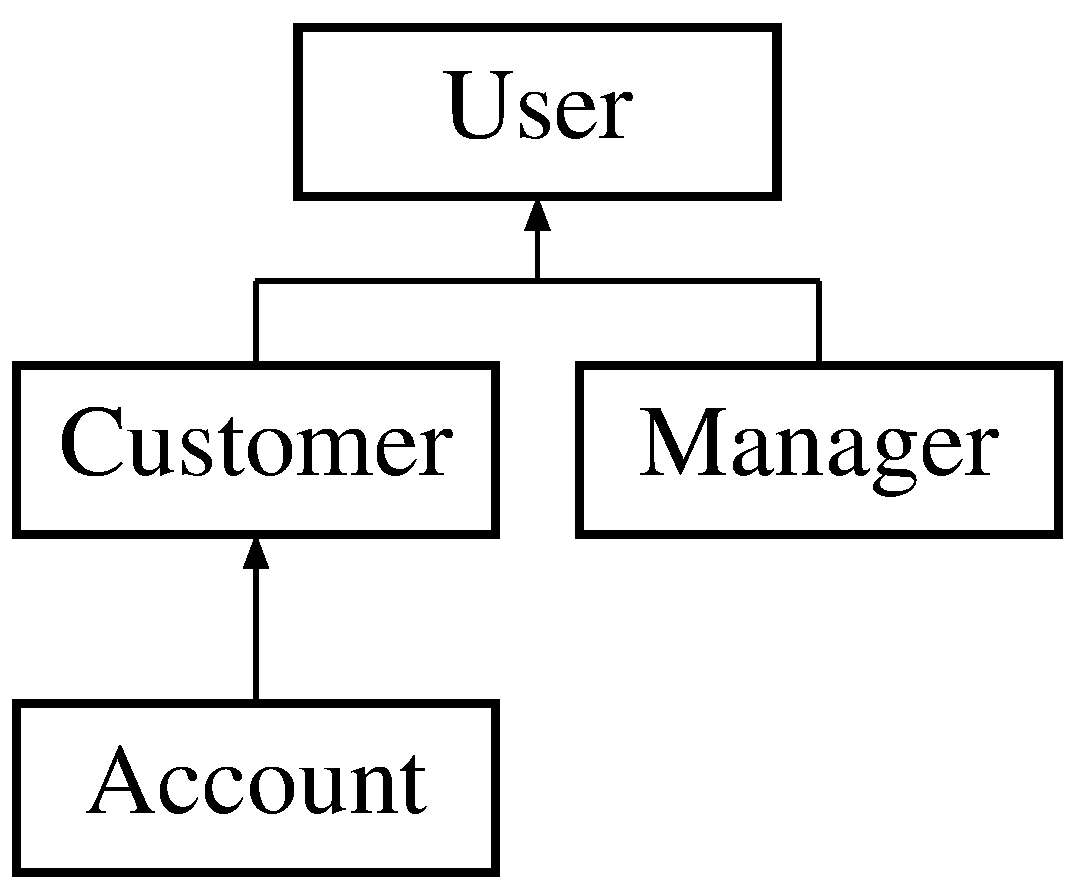
\includegraphics[height=2.000000cm]{d9/dc0/classUser}
\end{center}
\end{figure}
\subsubsection*{Public Member Functions}
\begin{DoxyCompactItemize}
\item 
\hyperlink{classUsrName}{Usr\-Name} \hyperlink{classUser_ae1dd9bb1a02ea1aa4246da19c28cd831}{get\-Name} () const 
\begin{DoxyCompactList}\small\item\em Método que recupera o valor contido no campo name. \end{DoxyCompactList}\item 
void \hyperlink{classUser_ac20aab332b1debfd3b94aa4fb7825b07}{set\-Usr\-Name} (const \hyperlink{classUsrName}{Usr\-Name} \&)
\begin{DoxyCompactList}\small\item\em Método que define o valor do atributo name. \end{DoxyCompactList}\item 
\hyperlink{classUsrPassword}{Usr\-Password} \hyperlink{classUser_a799c61fc6ff206a1b1edbc86d61989ed}{get\-Password} () const 
\begin{DoxyCompactList}\small\item\em Método que recupera o valor contido no campo password. \end{DoxyCompactList}\item 
void \hyperlink{classUser_ad36ece3d4decfd7f3db7f15c96eec99b}{set\-Usr\-Password} (const \hyperlink{classUsrPassword}{Usr\-Password} \&)
\begin{DoxyCompactList}\small\item\em Método que define o valor do atributo password. \end{DoxyCompactList}\end{DoxyCompactItemize}
\subsubsection*{Protected Attributes}
\begin{DoxyCompactItemize}
\item 
\hyperlink{classUsrName}{Usr\-Name} \hyperlink{classUser_a578e38a0fc23375ce19d689f96c6abaa}{name}
\begin{DoxyCompactList}\small\item\em Nome do usuário em questão. \end{DoxyCompactList}\item 
\hyperlink{classUsrPassword}{Usr\-Password} \hyperlink{classUser_a84c5ed822199a90e753ebfc54262fde8}{password}
\begin{DoxyCompactList}\small\item\em Senha do usuário em questão. \end{DoxyCompactList}\end{DoxyCompactItemize}


\subsubsection{Detailed Description}
Usuário; Base de derivação das classes \hyperlink{classCustomer}{Customer} e \hyperlink{classManager}{Manager}. 

Herdam dessa classe as duas maiores classes de usuários do sistema, os Clientes e os Gerentes. 

Definition at line 9 of file Entity\-Unit.\-h.



\subsubsection{Member Function Documentation}
\hypertarget{classUser_ae1dd9bb1a02ea1aa4246da19c28cd831}{\index{User@{User}!get\-Name@{get\-Name}}
\index{get\-Name@{get\-Name}!User@{User}}
\paragraph[{get\-Name}]{\setlength{\rightskip}{0pt plus 5cm}{\bf Usr\-Name} User\-::get\-Name (
\begin{DoxyParamCaption}
{}
\end{DoxyParamCaption}
) const\hspace{0.3cm}{\ttfamily [inline]}}}\label{d9/dc0/classUser_ae1dd9bb1a02ea1aa4246da19c28cd831}


Método que recupera o valor contido no campo name. 

O valor é retornado, e o atributo não é modificado no processo. 

Definition at line 29 of file Entity\-Unit.\-h.

\hypertarget{classUser_a799c61fc6ff206a1b1edbc86d61989ed}{\index{User@{User}!get\-Password@{get\-Password}}
\index{get\-Password@{get\-Password}!User@{User}}
\paragraph[{get\-Password}]{\setlength{\rightskip}{0pt plus 5cm}{\bf Usr\-Password} User\-::get\-Password (
\begin{DoxyParamCaption}
{}
\end{DoxyParamCaption}
) const\hspace{0.3cm}{\ttfamily [inline]}}}\label{d9/dc0/classUser_a799c61fc6ff206a1b1edbc86d61989ed}


Método que recupera o valor contido no campo password. 

O valor é retornado, e o atributo não é modificado no processo. 

Definition at line 33 of file Entity\-Unit.\-h.

\hypertarget{classUser_ac20aab332b1debfd3b94aa4fb7825b07}{\index{User@{User}!set\-Usr\-Name@{set\-Usr\-Name}}
\index{set\-Usr\-Name@{set\-Usr\-Name}!User@{User}}
\paragraph[{set\-Usr\-Name}]{\setlength{\rightskip}{0pt plus 5cm}void User\-::set\-Usr\-Name (
\begin{DoxyParamCaption}
\item[{const {\bf Usr\-Name} \&}]{name}
\end{DoxyParamCaption}
)}}\label{d9/dc0/classUser_ac20aab332b1debfd3b94aa4fb7825b07}


Método que define o valor do atributo name. 



Definition at line 7 of file Entity\-Unit.\-cpp.

\hypertarget{classUser_ad36ece3d4decfd7f3db7f15c96eec99b}{\index{User@{User}!set\-Usr\-Password@{set\-Usr\-Password}}
\index{set\-Usr\-Password@{set\-Usr\-Password}!User@{User}}
\paragraph[{set\-Usr\-Password}]{\setlength{\rightskip}{0pt plus 5cm}void User\-::set\-Usr\-Password (
\begin{DoxyParamCaption}
\item[{const {\bf Usr\-Password} \&}]{password}
\end{DoxyParamCaption}
)}}\label{d9/dc0/classUser_ad36ece3d4decfd7f3db7f15c96eec99b}


Método que define o valor do atributo password. 



Definition at line 11 of file Entity\-Unit.\-cpp.



\subsubsection{Member Data Documentation}
\hypertarget{classUser_a578e38a0fc23375ce19d689f96c6abaa}{\index{User@{User}!name@{name}}
\index{name@{name}!User@{User}}
\paragraph[{name}]{\setlength{\rightskip}{0pt plus 5cm}{\bf Usr\-Name} User\-::name\hspace{0.3cm}{\ttfamily [protected]}}}\label{d9/dc0/classUser_a578e38a0fc23375ce19d689f96c6abaa}


Nome do usuário em questão. 



Definition at line 12 of file Entity\-Unit.\-h.

\hypertarget{classUser_a84c5ed822199a90e753ebfc54262fde8}{\index{User@{User}!password@{password}}
\index{password@{password}!User@{User}}
\paragraph[{password}]{\setlength{\rightskip}{0pt plus 5cm}{\bf Usr\-Password} User\-::password\hspace{0.3cm}{\ttfamily [protected]}}}\label{d9/dc0/classUser_a84c5ed822199a90e753ebfc54262fde8}


Senha do usuário em questão. 



Definition at line 14 of file Entity\-Unit.\-h.



The documentation for this class was generated from the following files\-:\begin{DoxyCompactItemize}
\item 
Entity\-Unit.\-h\item 
Entity\-Unit.\-cpp\end{DoxyCompactItemize}

\hypertarget{classUsrId}{\section{Usr\-Id Class Reference}
\label{d8/dc7/classUsrId}\index{Usr\-Id@{Usr\-Id}}
}


Define o I\-D de um \hyperlink{classCustomer}{Customer}.  




{\ttfamily \#include $<$Base\-Unit.\-h$>$}

Inheritance diagram for Usr\-Id\-:\begin{figure}[H]
\begin{center}
\leavevmode
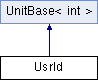
\includegraphics[height=2.000000cm]{d8/dc7/classUsrId}
\end{center}
\end{figure}
\subsection*{Public Member Functions}
\begin{DoxyCompactItemize}
\item 
\hyperlink{classUsrId_a55a05b8f951a218c66c49f09fa6ce374}{Usr\-Id} ()
\begin{DoxyCompactList}\small\item\em Construtor padrão de \hyperlink{classUsrId}{Usr\-Id}. \end{DoxyCompactList}\item 
\hyperlink{classUsrId_a3be81b6f539c0121803f9d88e9d89553}{Usr\-Id} (const int \&)  throw (invalid\-\_\-argument)
\begin{DoxyCompactList}\small\item\em Construtor base de \hyperlink{classUsrId}{Usr\-Id}. \end{DoxyCompactList}\end{DoxyCompactItemize}
\subsection*{Additional Inherited Members}


\subsection{Detailed Description}
Define o I\-D de um \hyperlink{classCustomer}{Customer}. 

Tem a função de identificar de forma única um \hyperlink{classCustomer}{Customer}, independentemente do seu tipo de conta. 

\subsection{Constructor \& Destructor Documentation}
\hypertarget{classUsrId_a55a05b8f951a218c66c49f09fa6ce374}{\index{Usr\-Id@{Usr\-Id}!Usr\-Id@{Usr\-Id}}
\index{Usr\-Id@{Usr\-Id}!UsrId@{Usr\-Id}}
\subsubsection[{Usr\-Id}]{\setlength{\rightskip}{0pt plus 5cm}Usr\-Id\-::\-Usr\-Id (
\begin{DoxyParamCaption}
{}
\end{DoxyParamCaption}
)}}\label{d8/dc7/classUsrId_a55a05b8f951a218c66c49f09fa6ce374}


Construtor padrão de \hyperlink{classUsrId}{Usr\-Id}. 

Define o valor 0 como valor de não-\/inicialização deste tipo básico. \hypertarget{classUsrId_a3be81b6f539c0121803f9d88e9d89553}{\index{Usr\-Id@{Usr\-Id}!Usr\-Id@{Usr\-Id}}
\index{Usr\-Id@{Usr\-Id}!UsrId@{Usr\-Id}}
\subsubsection[{Usr\-Id}]{\setlength{\rightskip}{0pt plus 5cm}Usr\-Id\-::\-Usr\-Id (
\begin{DoxyParamCaption}
\item[{const int \&}]{usr\-Id}
\end{DoxyParamCaption}
)  throw (invalid\-\_\-argument)}}\label{d8/dc7/classUsrId_a3be81b6f539c0121803f9d88e9d89553}


Construtor base de \hyperlink{classUsrId}{Usr\-Id}. 

É preferível que se utilize este construtor, pois ele já faz a validação automática do valor a ser definido. 

The documentation for this class was generated from the following files\-:\begin{DoxyCompactItemize}
\item 
Base\-Unit.\-h\item 
Base\-Unit.\-cpp\end{DoxyCompactItemize}

\hypertarget{classUsrMatric}{\section{Usr\-Matric Class Reference}
\label{classUsrMatric}\index{Usr\-Matric@{Usr\-Matric}}
}


Define a matrícula de um \hyperlink{classManager}{Manager}.  




{\ttfamily \#include $<$Base\-Unit.\-h$>$}

Inheritance diagram for Usr\-Matric\-:\begin{figure}[H]
\begin{center}
\leavevmode
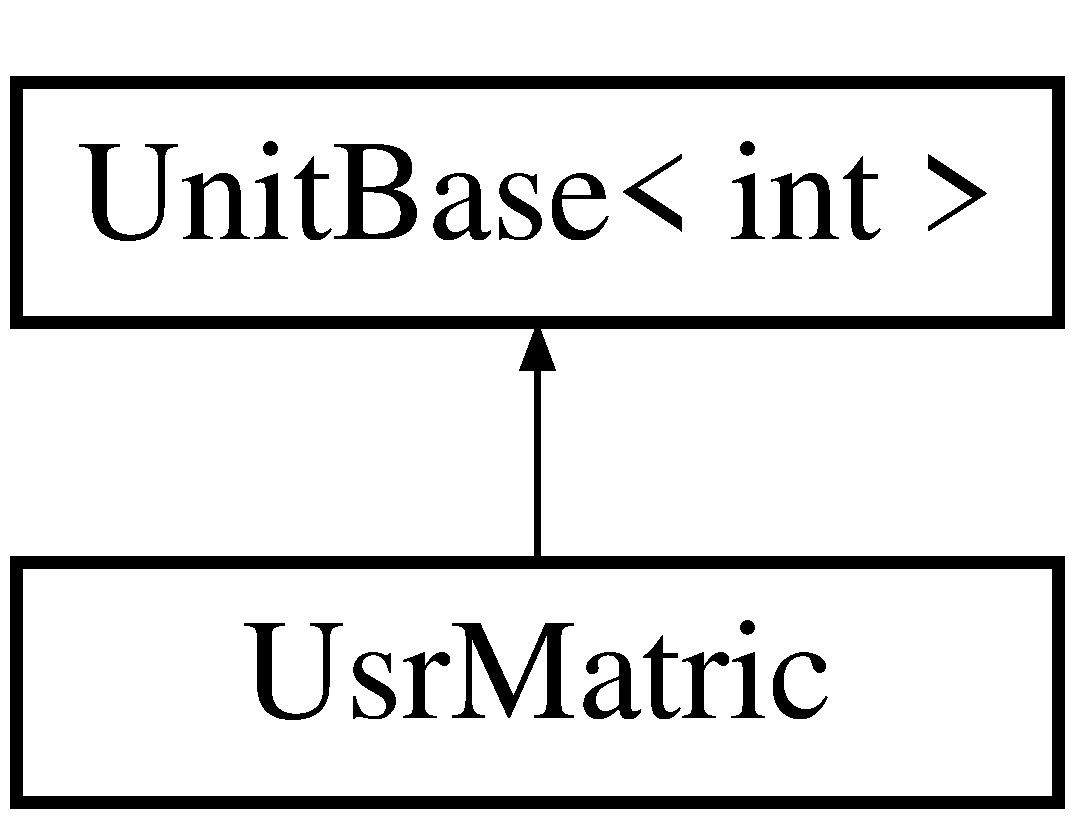
\includegraphics[height=2.000000cm]{classUsrMatric}
\end{center}
\end{figure}
\subsection*{Public Member Functions}
\begin{DoxyCompactItemize}
\item 
\hypertarget{classUsrMatric_acc7320dcfc8978fe9cc142340adb99c1}{{\bfseries Usr\-Matric} (const int \&)  throw (invalid\-\_\-argument)}\label{classUsrMatric_acc7320dcfc8978fe9cc142340adb99c1}

\end{DoxyCompactItemize}
\subsection*{Additional Inherited Members}


\subsection{Detailed Description}
Define a matrícula de um \hyperlink{classManager}{Manager}. 

Tem a função de identificar de forma única um \hyperlink{classManager}{Manager}, seja ele Administrador ou Gerente. 

The documentation for this class was generated from the following files\-:\begin{DoxyCompactItemize}
\item 
Base\-Unit.\-h\item 
Base\-Unit.\-cpp\end{DoxyCompactItemize}

\hypertarget{classUsrName}{\section{Usr\-Name Class Reference}
\label{da/df7/classUsrName}\index{Usr\-Name@{Usr\-Name}}
}


Define o nome de um \hyperlink{classUser}{User} (\hyperlink{classCustomer}{Customer} ou \hyperlink{classManager}{Manager}).  




{\ttfamily \#include $<$Base\-Unit.\-h$>$}

Inheritance diagram for Usr\-Name\-:\begin{figure}[H]
\begin{center}
\leavevmode
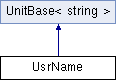
\includegraphics[height=2.000000cm]{da/df7/classUsrName}
\end{center}
\end{figure}
\subsection*{Public Member Functions}
\begin{DoxyCompactItemize}
\item 
\hyperlink{classUsrName_a0b0d5b9167309872d29c60a1946375af}{Usr\-Name} ()
\begin{DoxyCompactList}\small\item\em Construtor padrão de \hyperlink{classUsrName}{Usr\-Name}. \end{DoxyCompactList}\item 
\hyperlink{classUsrName_a3028672b21248ef880a01e3621e02827}{Usr\-Name} (const string \&)  throw (invalid\-\_\-argument)
\begin{DoxyCompactList}\small\item\em Construtor base de \hyperlink{classUsrName}{Usr\-Name}. \end{DoxyCompactList}\end{DoxyCompactItemize}
\subsection*{Additional Inherited Members}


\subsection{Detailed Description}
Define o nome de um \hyperlink{classUser}{User} (\hyperlink{classCustomer}{Customer} ou \hyperlink{classManager}{Manager}). 

Este tipo serve para regular o login de usuários em geral. 

\subsection{Constructor \& Destructor Documentation}
\hypertarget{classUsrName_a0b0d5b9167309872d29c60a1946375af}{\index{Usr\-Name@{Usr\-Name}!Usr\-Name@{Usr\-Name}}
\index{Usr\-Name@{Usr\-Name}!UsrName@{Usr\-Name}}
\subsubsection[{Usr\-Name}]{\setlength{\rightskip}{0pt plus 5cm}Usr\-Name\-::\-Usr\-Name (
\begin{DoxyParamCaption}
{}
\end{DoxyParamCaption}
)}}\label{da/df7/classUsrName_a0b0d5b9167309872d29c60a1946375af}


Construtor padrão de \hyperlink{classUsrName}{Usr\-Name}. 

Define a string vazia como valor de não-\/inicialização deste tipo básico \hypertarget{classUsrName_a3028672b21248ef880a01e3621e02827}{\index{Usr\-Name@{Usr\-Name}!Usr\-Name@{Usr\-Name}}
\index{Usr\-Name@{Usr\-Name}!UsrName@{Usr\-Name}}
\subsubsection[{Usr\-Name}]{\setlength{\rightskip}{0pt plus 5cm}Usr\-Name\-::\-Usr\-Name (
\begin{DoxyParamCaption}
\item[{const string \&}]{name}
\end{DoxyParamCaption}
)  throw (invalid\-\_\-argument)}}\label{da/df7/classUsrName_a3028672b21248ef880a01e3621e02827}


Construtor base de \hyperlink{classUsrName}{Usr\-Name}. 

É preferível que se utilize este construtor, pois ele já faz a validação automática do valor a ser definido. 

The documentation for this class was generated from the following files\-:\begin{DoxyCompactItemize}
\item 
Base\-Unit.\-h\item 
Base\-Unit.\-cpp\end{DoxyCompactItemize}

\hypertarget{classUsrPassword}{\section{Usr\-Password Class Reference}
\label{classUsrPassword}\index{Usr\-Password@{Usr\-Password}}
}


Define a senha de um \hyperlink{classUser}{User} (Customer ou \hyperlink{classManager}{Manager}).  




{\ttfamily \#include $<$Base\-Unit.\-h$>$}

Inheritance diagram for Usr\-Password\-:\begin{figure}[H]
\begin{center}
\leavevmode
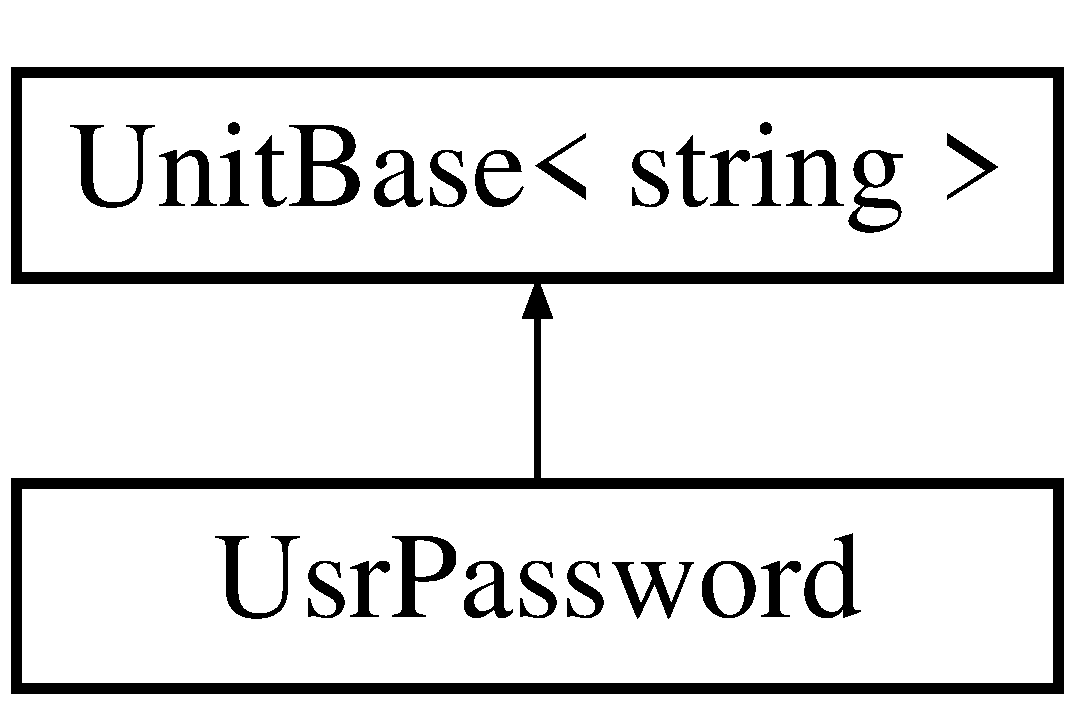
\includegraphics[height=2.000000cm]{classUsrPassword}
\end{center}
\end{figure}
\subsection*{Public Member Functions}
\begin{DoxyCompactItemize}
\item 
\hypertarget{classUsrPassword_ab99c93719778f9560712675b1febb3cb}{{\bfseries Usr\-Password} (const string \&)  throw (invalid\-\_\-argument)}\label{classUsrPassword_ab99c93719778f9560712675b1febb3cb}

\end{DoxyCompactItemize}
\subsection*{Additional Inherited Members}


\subsection{Detailed Description}
Define a senha de um \hyperlink{classUser}{User} (Customer ou \hyperlink{classManager}{Manager}). 

Este tipo básico tem a função de controlar o login de usuários em geral. 

The documentation for this class was generated from the following files\-:\begin{DoxyCompactItemize}
\item 
Base\-Unit.\-h\item 
Base\-Unit.\-cpp\end{DoxyCompactItemize}

\hypertarget{classUsrType}{\subsection{Usr\-Type Class Reference}
\label{d1/dd4/classUsrType}\index{Usr\-Type@{Usr\-Type}}
}


Codifica tipos de conta.  




{\ttfamily \#include $<$Base\-Unit.\-h$>$}

Inheritance diagram for Usr\-Type\-:\begin{figure}[H]
\begin{center}
\leavevmode
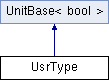
\includegraphics[height=2.000000cm]{d1/dd4/classUsrType}
\end{center}
\end{figure}
\subsubsection*{Public Member Functions}
\begin{DoxyCompactItemize}
\item 
\hyperlink{classUsrType_a51a73c6f2cfbca3174120a2796957c03}{Usr\-Type} ()
\begin{DoxyCompactList}\small\item\em Construtor padrão de \hyperlink{classUsrType}{Usr\-Type}. \end{DoxyCompactList}\item 
\hyperlink{classUsrType_a774f3a391ac5741802862cb7de682bb9}{Usr\-Type} (const bool \&)  throw (invalid\-\_\-argument)
\begin{DoxyCompactList}\small\item\em Construtor base de \hyperlink{classUsrType}{Usr\-Type}. \end{DoxyCompactList}\end{DoxyCompactItemize}
\subsubsection*{Additional Inherited Members}


\subsubsection{Detailed Description}
Codifica tipos de conta. 

Possui duas utilizações\-: Acc\-Type\-: Codifica tipos de conta (Normal / Especial) Man\-Type\-: Codifica tipos de manager (Gerente / Administrador) 

Definition at line 120 of file Base\-Unit.\-h.



\subsubsection{Constructor \& Destructor Documentation}
\hypertarget{classUsrType_a51a73c6f2cfbca3174120a2796957c03}{\index{Usr\-Type@{Usr\-Type}!Usr\-Type@{Usr\-Type}}
\index{Usr\-Type@{Usr\-Type}!UsrType@{Usr\-Type}}
\paragraph[{Usr\-Type}]{\setlength{\rightskip}{0pt plus 5cm}Usr\-Type\-::\-Usr\-Type (
\begin{DoxyParamCaption}
{}
\end{DoxyParamCaption}
)}}\label{d1/dd4/classUsrType_a51a73c6f2cfbca3174120a2796957c03}


Construtor padrão de \hyperlink{classUsrType}{Usr\-Type}. 

Define o valor N\-O\-R\-M\-A\-L/\-G\-E\-R\-E\-N\-T\-E como valor de não-\/inicialização deste tipo básico. 

Definition at line 90 of file Base\-Unit.\-cpp.

\hypertarget{classUsrType_a774f3a391ac5741802862cb7de682bb9}{\index{Usr\-Type@{Usr\-Type}!Usr\-Type@{Usr\-Type}}
\index{Usr\-Type@{Usr\-Type}!UsrType@{Usr\-Type}}
\paragraph[{Usr\-Type}]{\setlength{\rightskip}{0pt plus 5cm}Usr\-Type\-::\-Usr\-Type (
\begin{DoxyParamCaption}
\item[{const bool \&}]{usr\-Type}
\end{DoxyParamCaption}
)  throw (invalid\-\_\-argument)}}\label{d1/dd4/classUsrType_a774f3a391ac5741802862cb7de682bb9}


Construtor base de \hyperlink{classUsrType}{Usr\-Type}. 

É preferível que se utilize este construtor, pois ele já faz a validação automática do valor a ser definido. 

Definition at line 95 of file Base\-Unit.\-cpp.



The documentation for this class was generated from the following files\-:\begin{DoxyCompactItemize}
\item 
Base\-Unit.\-h\item 
Base\-Unit.\-cpp\end{DoxyCompactItemize}

\addcontentsline{toc}{part}{Index}
\printindex
\end{document}
